\documentclass{article}
\usepackage{amsmath, amssymb, amsthm, enumerate, framed, graphicx}
\usepackage[usenames,dvipsnames]{color}
\usepackage{bm}
\usepackage[colorlinks=true,urlcolor=blue]{hyperref}
\usepackage{geometry}
\geometry{margin=1in}
\usepackage{float}
\setlength{\marginparwidth}{2.15cm}
\usepackage{booktabs}
\usepackage{enumitem}
\usepackage{enumerate}
\usepackage{epsfig}
\usepackage{setspace}
\usepackage{parskip}
\usepackage{hyperref}
\usepackage[normalem]{ulem}
\usepackage{tikz}
\usepackage{pgfplots}
\usepackage[font=scriptsize]{subcaption}
\usepackage{float}
%\usepackage[]{algorithm2e}
\usepackage{environ}
\usepackage{bbm}
\usepackage[normalem]{ulem}
\usepackage{color}
\usepackage{minted}
\usepackage{tabu}
\usepackage[utf8]{inputenc}
\usepackage{array}
\usepackage{wrapfig}
\usepackage{multirow}
\usepackage[final]{listings}
\usepackage{algorithm}
\usepackage{algorithmicx}
\usepackage[noend]{algpseudocode}
\usepackage{datetime}
\usepackage{cancel}
\usepackage[many]{tcolorbox}
%\usepackage{xcolor}
\newcommand{\blackcircle}{\tikz\draw[black,fill=black] (0,0) circle (1ex);}
\renewcommand{\circle}{\tikz\draw[black] (0,0) circle (1ex);}

%%%%%%%%%%%%%%%%%%%%%%%%%%%%%%%%%%%%%%%%%%%
% Code highlighting with listings         %
%%%%%%%%%%%%%%%%%%%%%%%%%%%%%%%%%%%%%%%%%%%

\definecolor{bluekeywords}{rgb}{0.13,0.13,1}
\definecolor{greencomments}{rgb}{0,0.5,0}
\definecolor{redstrings}{rgb}{0.9,0,0}
\definecolor{light-gray}{gray}{0.95}

\newcommand{\MYhref}[3][blue]{\href{#2}{\color{#1}{#3}}}%

\definecolor{dkgreen}{rgb}{0,0.6,0}
\definecolor{gray}{rgb}{0.5,0.5,0.5}
\definecolor{mauve}{rgb}{0.58,0,0.82}

\lstdefinelanguage{Shell}{
  keywords={tar, cd, make},
  %keywordstyle=\color{bluekeywords}\bfseries,
  alsoletter={+},
  ndkeywords={python, py, javac, java, gcc, c, g++, cpp, .txt, octave, m, .tar},
  %ndkeywordstyle=\color{bluekeywords}\bfseries,
  identifierstyle=\color{black},
  sensitive=false,
  comment=[l]{//},
  morecomment=[s]{/*}{*/},
  commentstyle=\color{purple}\ttfamily,
  %stringstyle=\color{red}\ttfamily,
  morestring=[b]',
  morestring=[b]",
  backgroundcolor = \color{light-gray}
}

\lstset{columns=fixed, basicstyle=\ttfamily,
    backgroundcolor=\color{light-gray},xleftmargin=0.5cm,frame=tlbr,framesep=4pt,framerule=0pt}



%%%%%%%%%%%%%%%%%%%%%%%%%%%%%%%%%%%%%%%%%%%
% Custom box for highlights               %
%%%%%%%%%%%%%%%%%%%%%%%%%%%%%%%%%%%%%%%%%%%

% Define box and box title style
\tikzstyle{mybox} = [fill=blue!10, very thick,
    rectangle, rounded corners, inner sep=1em, inner ysep=1em]

\NewEnviron{notebox}{

\begin{tikzpicture}
\node [mybox] (box){
    \begin{minipage}{\textwidth}
        \BODY
    \end{minipage}
};
\end{tikzpicture}
}

\makeatletter
\newcommand{\removelatexerror}{\let\@latex@error\@gobble}
\makeatother

\newcommand{\argmax}{\mathop{\mathrm{argmax}}}
\newcommand{\argmin}{\mathop{\mathrm{argmin}}}
\newcommand{\Pb}{\mathbb{P}}
\newcommand{\xv}{\mathbf{x}}


\begin{document}

\section*{}
\begin{center}
  \centerline{\textsc{\LARGE Homework 7}}
  \vspace{0.5em}
  \centerline{\textsc{\LARGE MLE/MAP, Naive Bayes, Hidden Markov Models}}
  \vspace{1em}
  \textsc{\large CMU 10-601: Machine Learning (Fall 2019)} \\
  \url{}
  \centerline{OUT: 11/08/2019}
  \centerline{DUE: 11/25/2019 11:59 PM}
    \centerline{TAs: Anupma Sharan, Manini Amin, Bharath Prabhu, Max Le}
\end{center}

\begin{notebox}
\paragraph{Summary} This homework consists of 2 parts: The written section will review MLE/MAP, Naive Bayes, and HMM concepts. This section also includes some multiple choice warm-up problems to build your intuition for these models and then use that intuition to build your own HMM models. In the programming section, you will implement a new Named Entity Recognition system using Hidden Markov Models.
\end{notebox}

\section*{START HERE: Instructions\footnote{Compiled on \today{} at \currenttime{}}}
\begin{itemize}

\item \textbf{Collaboration Policy}: Collaboration on solving the homework is allowed, after you have thought about the problems on your own. It is also OK to get clarification (but not solutions) from books or online resources, again after you have thought about the problems on your own. There are two requirements: first, cite your collaborators fully and completely (e.g., ``Jane explained to me what is asked in Question 3.4''). Second, write your solution {\em independently}: close the book and all of your notes, and send collaborators out of the room, so that the solution comes from you only.  See the collaboration policy on the website for more information: \url{http://www.cs.cmu.edu/~mgormley/courses/10601/about.html}
\item\textbf{Late Submission Policy:} See the late submission policy
  here:
  \url{http://www.cs.cmu.edu/~mgormley/courses/10601/about.html}

\item\textbf{Submitting your work:} You will use Gradescope to submit
  answers to all questions, and Autolab to submit your code. Please
  follow instructions at the end of this PDF to correctly submit all your code to Autolab.

  \begin{itemize}
    
  % COMMENT IF NOT USING CANVAS
\begin{comment}
  \item \textbf{Canvas:} Canvas (\url{https://canvas.cmu.edu}) will be
    used for quiz-style problems (e.g. multiple choice, true / false,
    numerical answers). Grading is done automatically.
    %
    You may only \textbf{submit once} on canvas, so be sure of your
    answers before you submit. However, canvas allows you to work on
    your answers and then close out of the page and it will save your
    progress.  You will not be granted additional submissions, so
    please be confident of your solutions when you are submitting your
    assignment.
    %
    {\color{red} The above is true for future assignments, but this one
    allows {\bf unlimited submissions}.}
\end{comment}
    
  % COMMENT IF NOT USING GRADESCOPE
   \item \textbf{Gradescope:} For written problems such as derivations,
       proofs, or plots we will be using Gradescope
       (\url{https://gradescope.com/}). Submissions can be handwritten, but
       should be labeled and clearly legible. If your writing is not
       legible, you will not be awarded marks. Alternatively, submissions
       can be written in LaTeX. Upon submission, label each question
       using the template provided. Regrade requests can be made, however
       this gives the TA the opportunity to regrade your entire paper,
       meaning if additional mistakes are found then points will be
       deducted.
       %   
       Each derivation/proof should be  completed on a separate page.

  %   COMMENT IF NOT USING AUTOLAB
  \item \textbf{Autolab:} You will submit your code for programming
    questions on the homework to Autolab
    (\url{https://autolab.andrew.cmu.edu/}). After uploading your code,
    our grading scripts will autograde your assignment by running your
    program on a virtual machine (VM). 
    %
    The software installed on the VM is identical to that on
    \texttt{linux.andrew.cmu.edu}, so you should check that your code
    runs correctly there. If developing locally, check that the
    version number of the programming language environment
    (e.g. Python 2.7, Octave 3.8.2, OpenJDK 1.8.0, g++ 4.8.5) and
    versions of permitted libraries (e.g. \texttt{numpy} 1.7.1) match
    those on \texttt{linux.andrew.cmu.edu}.
    % 
    Octave users: Please make sure you do not use any
    Matlab-specific libraries in your code that might make it fail
    against our tests.
    %
    Python3 users: Please include a blank file called python3.txt (case-sensitive) in your tar submission. 
    %
    You have a {\bf total of 10 Autolab submissions}. Use them
    wisely. In order to not waste Autolab submissions, we recommend
    debugging your implementation on your local machine (or the linux
    servers) and making sure your code is running correctly first
    before any Autolab submission. 
    %

  \end{itemize}
  
\item\textbf{Materials:} Download from autolab the tar file ("Download
  handout"). The tar file will contain all the data that you will need in order to complete this assignment.

\end{itemize}

For multiple choice or select all that apply questions, shade in the box or circle in the template document corresponding to the correct answer(s) for each of the questions. For \LaTeX users, use $\blacksquare$ and $\blackcircle$  for shaded boxes and circles, and don't change anything else.

\clearpage

\section*{Instructions for Specific Problem Types}

For ``Select One" questions, please fill in the appropriate bubble completely:

\begin{quote}
\textbf{Select One:} Who taught this course?
\begin{list}{}
     \item $\blackcircle$ Matt Gormley
     \item $\circle$ Marie Curie
     \item $\circle$ Noam Chomsky
\end{list}
\end{quote}

If you need to change your answer, you may cross out the previous answer and bubble in the new answer:

\begin{quote}
\textbf{Select One:} Who taught this course?
\begin{list}{}
     \item $\blackcircle$ Matt Gormley
     \item $\circle$ Marie Curie\\
     \xcancel{$\blackcircle$}{} Noam Chomsky
\end{list}
\end{quote}


For ``Select all that apply" questions, please fill in all appropriate squares completely:

\begin{quote}
\textbf{Select all that apply:} Which are scientists?
    \begin{list}{}
    \item $\blacksquare$ Stephen Hawking 
    \item $\blacksquare$ Albert Einstein
    \item $\blacksquare$ Isaac Newton
    \item $\square$ I don't know
\end{list}
\end{quote}

Again, if you need to change your answer, you may cross out the previous answer(s) and bubble in the new answer(s):

\begin{quote}
\textbf{Select all that apply:} Which are scientists?
    \begin{list}{}
    \item $\blacksquare$ Stephen Hawking 
    \item $\blacksquare$ Albert Einstein
    \item $\blacksquare$ Isaac Newton\\
    \xcancel{$\blacksquare$} I don't know
\end{list}
\end{quote}

For questions where you must fill in a blank, please make sure your final answer is fully included in the given space. You may cross out answers or parts of answers, but the final answer must still be within the given space.

\begin{quote}
\textbf{Fill in the blank:} What is the course number?

\begin{tcolorbox}[fit,height=1cm, width=4cm, blank, borderline={1pt}{-2pt},nobeforeafter]
    \begin{center}\huge10-601\end{center}
    \end{tcolorbox}\hspace{2cm}
    \begin{tcolorbox}[fit,height=1cm, width=4cm, blank, borderline={1pt}{-2pt},nobeforeafter]
    \begin{center}\huge10-\xcancel{7}601\end{center}
    \end{tcolorbox}
\end{quote}


\clearpage


\section{MLE/MAP [22 pts]}
\begin{enumerate}


    \item \textbf{[1 pt]} \textbf{True or False:} Suppose you place a Beta prior over the Bernoulli distribution, and attempt to learn the parameter of the Bernoulli distribution from data. Further suppose an adversary chooses ``bad", but finite hyperparameters for your Beta prior in order to confuse your learning algorithm. As the number of training examples grows to infinity, the MAP estimate of $\theta$ can still converge to the MLE estimate of $\theta$.
    
    \textbf{Select One:}
    
    \begin{list}{}
        \item $\circle$ True
        \item $\circle$ False
    \end{list}
    
    \item \textbf{[3 pt]} In HW3, you have derived the closed form solution for linear regression. Now, we are coming back to linear regression, viewing it as a statistical model, and deriving the MLE and MAP estimate of the parameters in the following questions. 
    
    Assume we have data $D = \{\mathbf{x}^{(i)}, y^{(i)}\}_{i=1}^{N}$, where $\mathbf{x}^{(i)} = (x_1^{(i)}, \cdots, x_M^{(i)})$ . So our data has $N$  instances and each instance has $M$  attributes/features. Each $y^{(i)}$ is generated given $\mathbf{x}^{(i)}$ with additive noise $\epsilon^{(i)} \sim N(0, \sigma^2)$, that is $y^{(i)} = \mathbf{w}^T \mathbf{x}^{(i)} + \epsilon^{(i)}$ where $\mathbf{w}$  is the parameter vector of linear regression. Given this assumption, what is the distribution of y? 

    \textbf{Select one:}
    \begin{list}{}
        \item $\circle$ $y^{(i)} \sim N(\mathbf{w}^T \mathbf{x}^{(i)}, \sigma^2)$
        \item $\circle$ $y^{(i)} \sim N(0, \sigma^2)$
        \item $\circle$ $y^{(i)} \sim \textit{Uniform}(\mathbf{w}^T \mathbf{x}^{(i)} - \sigma,  \mathbf{w}^T \mathbf{x}^{(i)} + \sigma)$
        \item $\circle$ None of the above
    \end{list}
    
    \item \textbf{[3 pt]} The next step is to learn the MLE of the parameters of the linear regression model. Which expression below is the correct conditional log likelihood $\ell(\mathbf{w})$ with the given data?

    \textbf{Select one:}
    \begin{list}{}
        \item $\circle$ $\sum_{i=1}^{N} [-\log (\sqrt{2\pi\sigma^2}) - \frac{1}{2\sigma^2} (y^{(i)} - \mathbf{w}^T\mathbf{x}^{(i)})^2]$
        \item $\circle$ $\sum_{i=1}^{N} [\log (\sqrt{2\pi\sigma^2}) + \frac{1}{2\sigma^2} (y^{(i)} - \mathbf{w}^T\mathbf{x}^{(i)})^2]$
        \item $\circle$ $\sum_{i=1}^{N} [-\log(\sqrt{2\pi\sigma^2)} - \frac{1}{2\sigma^2} (y^{(i)} - \mathbf{w}^T\mathbf{x}^{(i)})]$
        \item $\circle$ $-\log (\sqrt{2\pi\sigma^2}) + \sum_{i=1}^{N} [-\frac{1}{2\sigma^2} (y^{(i)} - \mathbf{w}^T\mathbf{x}^{(i)})^2]$
    \end{list}
    
    \item \textbf{[4 pt]} Then, the MLE of the parameters is just  $\argmax_{\mathbf{w}} \ell(\mathbf{w})$ . Among the following expressions, select ALL that can yield the correct MLE. 

    \textbf{Select all that apply:}
    \begin{list}{}
        \item $\square$ $\argmax_{\mathbf{w}} \sum_{i=1}^{N} [-\log (\sqrt{2\pi\sigma^2}) - \frac{1}{2\sigma^2} (y^{(i)} - \mathbf{w}^T\mathbf{x}^{(i)})]$
        \item $\square$ $\argmax_{\mathbf{w}} \sum_{i=1}^{N} [-\log (\sqrt{2\pi\sigma^2}) - \frac{1}{2\sigma^2} (y^{(i)} - \mathbf{w}^T\mathbf{x}^{(i)})^2]$
        \item $\square$ $\argmax_{\mathbf{w}} \sum_{i=1}^{N} [- \frac{1}{2\sigma^2} (y^{(i)} - \mathbf{w}^T\mathbf{x}^{(i)})^2]$
        \item $\square$ $\argmax_{\mathbf{w}} \sum_{i=1}^{N} [- \frac{1}{2} (y^{(i)} - \mathbf{w}^T\mathbf{x}^{(i)})]$
        \item $\square$ $\argmax_{\mathbf{w}} \sum_{i=1}^{N} [- \frac{1}{2} (y^{(i)} - \mathbf{w}^T\mathbf{x}^{(i)})^2]$
    \end{list}
    
    \item \textbf{[3 pt]} Now we are moving on to learn the MAP estimate of the parameters of the linear regression model. The MAP estimate is obtained through solving the following optimization problem.

    $\mathbf{w}_{MAP} = \arg\max_{\mathbf{w}} p(\mathbf{w} | D) = \arg\max_{\mathbf{w}} p(D, \mathbf{w})$

    Suppose are using a Gaussian prior distribution with mean 0 and variance $\frac{1}{\lambda}$ for each element $w_m$  of the parameter vector $\mathbf{w} (1 \leq m \leq M $), i.e. $w_m \sim N(0, \frac{1}{\lambda})$. Assume that $w_1, \cdots, w_M$ are mutually independent of each other. Which expression below is the correct log joint-probability of the data and parameters $\log p(D, \mathbf{w}))$? 

    (For simplicity, just use $p(D|\mathbf{w})$ to denote the data likelihood.)

    \textbf{Select one:}
    \begin{list}{}
        \item $\circle$ $\log p(D|\textbf{w}) - \sum_{m=1}^M \log(\sqrt{2\pi\lambda}) - \lambda (w_m)^2$
        \item $\circle$ $\log p(D|\textbf{w}) + \sum_{m=1}^M -\log(\sqrt{2\pi\lambda}) - \lambda (w_m)^2$
        \item $\circle$ $\log p(D|\textbf{w}) -  \sum_{m=1}^M \log(\sqrt{\frac{2\pi}{\lambda}}) - \frac{\lambda}{2}(w_m)^2$
        \item $\circle$ $\log p(D|\textbf{w}) +  \sum_{m=1}^M -\log(\sqrt{\frac{2\pi}{\lambda}}) - \frac{\lambda}{2}(w_m)^2$
    \end{list}
    
    \item \textbf{[2 pt]} A MAP estimator with a Gaussian prior $\mathcal{N}(0, \sigma^2)$ you trained gives significantly higher test error than train error. What could be a possible approach to fixing this? 

    \textbf{Select one:}
    \begin{list}{}
        \item $\circle$ Increase variance $\sigma^2$
        \item $\circle$ Decrease variance $\sigma^2$
        \item $\circle$ Try MLE estimator instead
        \item $\circle$ None of the above
    \end{list}
    
    \item \textbf{[3 pt]} Maximizing the log posterior probability  $\ell_{\textit{MAP}}(\mathbf{w})$ gives you the MAP estimate of the parameters. The MAP estimate with Gaussian prior is actually equivalent to a L2 regularization on the parameters of linear regression model in minimizing an objective function $J(\mathbf{w})$ that consists of a term related to log conditional likelihood $\ell(\mathbf{w})$ and a L2 regularization term. The following options specify the two terms in $J(\mathbf{w})$ explicitly. Which one is correct based on your derived log posterior probability in the previous question? 

    \textbf{Select one:}
    \begin{list}{}
        \item $\circle$ $- \ell(\mathbf{w}) + \frac{\lambda}{2}\|\mathbf{w}\|_2$
        \item $\circle$ $- \ell(\mathbf{w}) + \frac{\lambda}{2}\|\mathbf{w}\|_2^2$
        \item $\circle$ $- \ell(\mathbf{w}) + \lambda\|\mathbf{w}\|_2$
        \item $\circle$ $\ell(\mathbf{w}) - \frac{\lambda}{2}\|\mathbf{w}\|_2^2$
    \end{list}
    
    \clearpage
    
    \item \textbf{[3 pt]} MAP estimation with what prior is equivalent to L1 regularization? 

    Note:\\
    The pdf of a Uniform distribution over [a,b] is $f(x) = \frac{1}{b-a}$ if $x \in [a,b]$ and 0 otherwise.\\
    The pdf of an exponential distribution with rate parameter $a$ is $f(x) = a \exp(-a x)$ for $x > 0$.\\
    The pdf of a Laplace distribution with location parameter $a$ and scale parameter $b$  is $f(x) = \frac{1}{2b} \exp \left( \frac{- |x - a| }{b} \right)$ for all $x \in \mathbb{R}$.
    

    \textbf{Select one:}
    \begin{list}{}
        \item $\circle$ Uniform distribution over $[- \mathbf{w}^T\mathbf{x}^{(i)}, \mathbf{w}^T\mathbf{x}^{(i)} ]$
        \item $\circle$ Exponential distribution with rate parameter $a = \frac{1}{2}$
        \item $\circle$ Exponential distribution with rate parameter $a = \mathbf{w}^T \mathbf{x}^{(i)}$
        \item $\circle$ Laplace prior with location parameter $a = 0$
        \item $\circle$ Laplace prior with location parameter $a = \mathbf{w}^T \mathbf{x}^{(i)}$
        \item $\circle$ Uniform distribution over [-1, 1]
    \end{list}
    
\end{enumerate}

\clearpage

\section{Naive Bayes [13 pts]}
\begin{enumerate}

    \item \textbf{[2 pt]} If I give you for events A and B, $P(A\mid B) = 2/3$, $P(A\mid \neg B) = 1/3$ and $P(B) = 1/3$ and $P(A) = 4/9$, where $\neg B$ denotes the complement of B. Do you have information to calculate $P(B\mid A)$? If not, choose ``not enough information", if so, compute the value of $P(B\mid A)$.

    \textbf{Select one:}
    \begin{list}{}
        \item $\circle$ 1/2
        \item $\circle$ 2/3
        \item $\circle$ 1/3
        \item $\circle$ Not enough information
    \end{list}
    
    \item \textbf{[3 pt]} Gaussian Naive Bayes in general can learn non-linear decision boundaries. Consider the simple case where we have just one real-valued feature $X_1\in\mathbb{R}$ from which we wish to infer the value of label $Y\in\{0,1\}$.The corresponding generative story would be:
    
    $Y \sim \text{Bernoulli}(\phi)$\\
    $X_1 \sim \text{Gaussian}(\mu_y, \sigma^2_y)$\\
    where the parameters are the Bernoulli parameter $\phi$  and the class-conditional Gaussian parameters $\mu_0, \sigma^2_0$ and $\mu_1, \sigma^2_1$   corresponding to $Y=0$ and $Y=1$ , respectively.

    A linear decision boundary in one dimension, of course, can be described by a rule of the form ``if $X_1>c$  then $Y=1$, else $Y=0$", where $c$ is a real-valued threshold (see diagram provided). Is it possible in this simple one-dimensional case to construct a Gaussian Naive Bayes classifier with a decision boundary that cannot be expressed by a rule in the above form)?

    \begin{figure}[H]
        \centering
        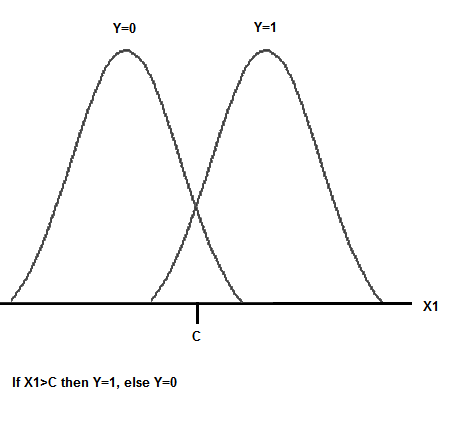
\includegraphics[width=0.4\textwidth]{Gaussians.png}
    \end{figure}
    \textbf{Select one:}
    \begin{list}{}
        \item $\circle$ Yes, this can occur if the Gaussians are of equal means and equal variances.
        \item $\circle$ Yes, this can occur if the Gaussians are of equal means and unequal variances.
        \item $\circle$ Yes, this can occur if the Gaussians are of unequal means and equal variances. 
        \item $\circle$ No, this cannot occur regardless of the relationship of the means or variances.
    \end{list}
    
    \clearpage

    \item \textbf{[3 pt]} Suppose that $0.3\%$ people have cancer. Someone decided to take a medical test for cancer. The outcome of the test can either be positive (cancer) or negative (no cancer). The test is not perfect - among people who have cancer, the test comes back positive 97\% of the time. Among people who don’t have cancer, the test comes back positive 4\% of the time. For this question, you should assume that the test results are independent of each other, given the true state (cancer or no cancer). What is the probability of a test subject having cancer, given that the subject’s test result is positive?
    
    If your answer is in decimals, answer with precision 4, e.g. (6.051, 0.1230, 1.234e+7)

    \textbf{Fill in the blank:}
    
    \begin{tcolorbox}[fit,height=1cm, width=4cm, blank, borderline={1pt}{-2pt},nobeforeafter]
    
    %solution
    \end{tcolorbox}
    
    \item \textbf{[2 pt]} In a Naive Bayes problem, suppose we are trying to compute $P(Y\mid X_1,X_2,X_3,X_4)$ .  Furthermore, suppose  $X_2$  and  $X_3$  are identical (i.e., $X_3$  is just a copy of $X_2$ ).  Which of the following are true in this case?

    \textbf{Select all that apply:}
    \begin{list}{}
        \item $\square$ Naive Bayes will learn identical parameter values for $P(X_2|Y)$ and $P(X_3|Y)$.
        \item $\square$ Naive Bayes will output probabilities $P(Y|X_1,X_2,X_3,X_4)$ that are closer to 0 and 1 than they would be if we removed the feature corresponding to $X_3$.
        \item $\square$ This will not raise a problem in the output  $P(Y|X_1,X_2,X_3,X_4)$ because the conditional independence assumption will correctly treat this situation.
        \item $\square$ None of the above
    \end{list}
    
    \item \textbf{[3 pt]} Which of the following machine learning algorithms are probabilistic generative models? 

    \textbf{Select all that apply:}
    \begin{list}{}
        \item $\square$ Decision Tree
        \item $\square$ K-nearest neighbors
        \item $\square$ Perceptron
        \item $\square$ Naive Bayes
        \item $\square$ Logistic Regression
        \item $\square$ Feed-forward neural network
    \end{list}

\end{enumerate}

\clearpage

\section{Written Questions [15 pts]}
\subsection{Multiple Choice [4 pts]}
In this section we will test your understanding of several aspects of HMMs.
%
Shade in the box or circle in the template document corresponding to the correct answer(s) for each of the questions below. 


\begin{enumerate}
\item \textbf{[2 pts, Select all that apply]} Which of the following are true under the (first-order) Markov assumption in an HMM: 
\begin{list}{$\square$}{}
\item The states are independent
\item The observations are independent
\item $y_t \perp y_{t-1} | y_{t-2}$
\item $y_t \perp y_{t-2} | y_{t-1}$
\item None of the above
\end{list}


\item \textbf{[2 pts, Select all that apply]} Which of the following independence assumptions hold in an HMM:
\begin{list}{$\square$}{}
\setlength\itemsep{-1.5em}
\item The current observation $x_t$ is conditionally independent of all other observations given the current state $y_t$\\
\item The current observation $x_t$ is conditionally independent of all other states given the current state $y_t$\\
\item The current state $y_t$ is conditionally independent of all states given the previous state $y_{t-1}$\\
\item The current observation $x_t$ is conditionally independent of $x_{t-2}$ given the previous observation $x_{t-1}$.\\
\item None of the above
\end{list}

\end{enumerate}


\subsection{Warm-up Exercise: Viterbi Algorithm [5 pts]}\label{toy}
% working example [4 points]
% write the example
To help you prepare to implement the HMM Viterbi algorithm (see Section~\ref{viterbi} for a detailed explanation), we have provided a small example for you to work through by hand. This toy data set consists of a training set of three sequences with three unique words and two tags and a test set with a single sequence composed of the same unique words used in the training set. Before going through this example, please carefully read the algorithm description in Sections \ref{learn} and \ref{viterbi}.

Training set:
\begin{verbatim}
you_B eat_A fish_B
you_B fish_B eat_A
eat_A fish_B
\end{verbatim}

Where the training word sequences are:
$$
x= 
\begin{bmatrix}
you & eat & fish\\
you & fish & eat\\
eat & fish &
\end{bmatrix}
$$

And the corresponding tags are:
$$
y= 
\begin{bmatrix}
B & A & B\\
B & B & A\\
A & B &
\end{bmatrix}
$$


Test set:
\begin{verbatim}
fish eat you
\end{verbatim}

or 

$$
x= 
\begin{bmatrix}
fish & eat & you\\
\end{bmatrix}
$$

The following questions are meant to encourage you to work through the Viterbi algorithm by hand using this test example. Here we perform Viterbi decoding on the \textbf{test set}. We use the same notations defined in section \ref{viterbi}: $w_t(j)$ is the highest probability path ending at state $s_j$ at time $t$ (eg $y_t = s_j$).

Feel free to use a calculator, being careful to carry enough significant figures through your computations to avoid rounding errors. For each question below, please report the requested value in the text box next to the question (these boxes are only visible in the template document). When a number is requested, only write the number in the box. When a word/tag is requested, only write that word or tag. \textbf{DO NOT} include explanations or derivation work in the text box. Points will be deducted if anything else is included in the box.

\begin{enumerate}

    \item \textbf{[0 pt]} To help you compute the subsequent questions, we suggest you write down the initial probabilities $\pi$, transition probabilities $\textbf{B}$, and emission probabilities $\textbf{A}$, as defined in section \ref{learn}. The solutions are already given in the handout. Note that the probabilities $\textbf{A}$, $\textbf{B}$ are different from the tags \texttt{A}, \texttt{B}
    
    \item \textbf{[1 pt]} Compute $w_1(\texttt{A})$.
    
    \begin{tcolorbox}[fit,height=1cm, width=2cm, blank, borderline={1pt}{-2pt}]
            %solution 
        \end{tcolorbox}
    
    \item \textbf{[1 pt]} Compute $w_2(\texttt{A})$
    
    \begin{tcolorbox}[fit,height=1cm, width=2cm, blank, borderline={1pt}{-2pt}]
            %solution 
        \end{tcolorbox}
    
    \item \textbf{[1 pt]} If you predict that $y_2 = \texttt{A}$, what will be $y_1$ (tag at step $t = 1$)? 
    
    \begin{tcolorbox}[fit,height=1cm, width=2cm, blank, borderline={1pt}{-2pt}]
            %solution 
        \end{tcolorbox}
    
    \item \textbf{[1 pt]} Compute $w_3(\texttt{B})$
    
    \begin{tcolorbox}[fit,height=1cm, width=2cm, blank, borderline={1pt}{-2pt}]
            %solution 
        \end{tcolorbox}
    
    \item \textbf{[1 pt]} If you predict that $y_3 = \texttt{B}$, what will be $y_2$ (tag at step $t = 2$)?
    
    \begin{tcolorbox}[fit,height=1cm, width=2cm, blank, borderline={1pt}{-2pt}]
            %solution 
        \end{tcolorbox}
    
    \item \textbf{[0 pt]} What is your final predicted tag sequence for test set? You should check that this match with the \texttt{predictedtest.txt} file for toy dataset we gave you in the handout.
    
\end{enumerate}

\clearpage

\subsection{Empirical Questions [6 pts]}
[Return to these questions after implementing your \texttt{learnhmm.\{py|java|cpp|m\}} and \texttt{viterbi.\{py|java|cpp|m\}} functions]

Using the fulldata set \textbf{trainwords.txt} in the handout using your implementation of \texttt{learnhmm.\{py|java|cpp|m\}} to learn parameters for an hmm model using the first 10, 100, 1000, and 10000 sequences in the file.
Use these learned parameters perform prediction on the \textbf{trainwords.txt} and the \textbf{testwords.txt} files using your \texttt{viterbi.\{py|java|cpp|m\}}.
Construct a plot with number of sequences used for training on the x-axis and accuracy of all sequences from the \textbf{trainwords.txt} or the \textbf{testwords.txt} on the y-axis (see Section~\ref{forback} for details on computing the log data likelihood for a sequence). Each table entry is worth 0.5 points. 
Write the resulting accuracy values in the table in the template.
Include your plot in the large box in the template (2 points).
To receive credit for your plot, you must submit a computer generated plot.
\textbf{DO NOT} hand draw your plot.

\begin{table}[h]
    \center
    \begin{tabular}{|m{2cm}|m{3cm}|m{3cm}|}
    \hline
    \#sequences & Train accuracy & Test accuracy \\ \hline
    10         &    &  \\ \hline
    100        &    &  \\ \hline
    1000       &    &  \\ \hline
    10000      &    &  \\ \hline
    \end{tabular}
    \end{table}

 \begin{tcolorbox}[fit,height=13cm, width=17cm, blank, borderline={1pt}{-2pt}]
    %solution 
 \end{tcolorbox}

\subsection{Collaboration Policy}
After you have completed all other components of this assignment, report your answers to the collaboration policy questions detailed in the Academic Integrity Policies found \href{http://www.cs.cmu.edu/~mgormley/courses/10601bd-f18/about.html#7-academic-integrity-policies}{here}.
    \begin{enumerate}
        \item Did you receive any help whatsoever from anyone in solving this assignment? Is so, include full details.
        \item Did you give any help whatsoever to anyone in solving this assignment? Is so, include full details.
        \item Did you find or come across code that implements any part of this assignment ? If so, include full details.
    \end{enumerate}

\begin{tcolorbox}[fit,height=10cm, width=17cm, blank, borderline={1pt}{-2pt}]
    %solution 
    \end{tcolorbox}

\clearpage


\section{Programming [50 pts]}
\label{programming}

\subsection{The Tasks and Data Sets}\label{dataset}
The handout file for this assignments contains several files that you will use in the homework. The contents and formatting of each of these files is explained below.
\begin{enumerate}

\item \textbf{trainwords.txt} This file contains labeled text data that you will use in training your model in the \textbf{Learning} problem. Specifically the text contains one sentence per line that has already been preprocessed, cleaned and tokenized. You should treat every line as a separate sequence and assume that it has the following format:

    \texttt{<Word0>\_<Tag0> <Word1>\_<Tag1> ... <WordN>\_<TagN>}

where every \texttt{<WordK>\_<TagK>} unit token is separated by white space.

\item \textbf{testwords.txt}: This file contains labeled data that you will use to evaluate your model. This file has the same format as \textbf{trainwords.txt}.
    
\item \textbf{index\_to\_word.txt} and \textbf{index\_to\_tag.txt}: These files contain a list of all words or tags that appear in the data set. In your functions, you will convert the string representation of words or tags to indices corresponding to the location of the word or tag in these files. For example, if Austria is on line 729 of \textbf{index\_to\_word.txt}, then all appearances of Austria in the data sets should be converted to the index 729. This index will also correspond to locations in the parameter matrices. For example, the word Austria corresponds to the parameters in column 729 of the matrix stored in \textbf{hmmemit.txt}.

\item \textbf{predictedtest.txt} This file contains labeled data that you will use to debug your implementation. The labels in this file are not gold standard but are generated by running our decoder on \textbf{testwords.txt}. This file has the same format as \textbf{testwords.txt}.

\item \textbf{metrics.txt} This file contains the metrics you will compute for the dataset. For this assignment, you need to compute prediction accuracy on the test data. Note that in Named Entity Recognition, F-1 score is a more common metric to evaluate the model performance, here you only need to report your accuracy for tag prediction of each word.

\item \textbf{hmmtrans.txt, hmmemit.txt and hmmprior.txt}: These files contain pre-trained model parameters of an HMM that you will use in testing your implementation of the \textbf{Learning} and \textbf{Decoding} problems. The format of the first two files are analogous and is as follows. Every line in these files consists of a conditional probability distribution. In the case of transition probabilities, this distribution corresponds to the probability of transitioning into another state, given a current state. Similarly, in the case of emission probabilities, this distribution corresponds to the probability of emitting a particular symbol, given a current state. For example, every line in \textbf{hmmtrans.txt} has the following format:
    
    \textbf{hmmtrans.txt}:\\
    \texttt{<ProbS1S1> ... <ProbS1SN>}\\
     \texttt{<ProbS2S1> ... <ProbS2SN>}...\\   
    
and every line in \textbf{hmmemit.txt} has the following format:
    
    \textbf{hmmemit.txt}:\\
    \texttt{<ProbS1Word1> ... <ProbS1WordN>}\\
     \texttt{<ProbS2Word1> ... <ProbS2WordN>}...\\
    
In both cases, elements in the same row are separated by white space. Each row corresponds to a line of text (using \texttt{\char`\\ n} to create new lines).
    
    
The format of \textbf{hmmprior.txt} is similarly defined except that it only contains a single probability distribution over starting states. Therefore each row only has a single element. Therefore \textbf{hmmprior.txt} has the following format:
    
    \textbf{hmmprior.txt}:\\
    \texttt{<ProbS1>}\\
     \texttt{<ProbS2>}...\\

\item \textbf{toytrain.txt}, \textbf{toytest.txt}, \textbf{toy\_index\_to\_word.txt}, \textbf{toy\_index\_to\_tag.txt}: These files are analogous to \textbf{trainwords.txt}, \textbf{testwords.txt}, \textbf{index\_to\_word.txt}, and \textbf{index\_to\_tag.txt}. We also give you \textbf{hmmprior.txt}, \textbf{hmmemit.txt}, \textbf{hmmtrans.txt}, \textbf{predictedtext.txt}, and \textbf{metrics.txt} of the toy dataset that you can use for debugging. You should also use them to compare your implementation to your hand calculations in Section~\ref{toy}.
\end{enumerate}

Note that the data provided to you is to help in developing your implementation of the HMM algorithms. Your code will be tested on Autolab using different data with different HMM parameters, likely coming from a different domain although the format will be identical.

\subsection{Learning}\label{learn}
Your first task is to implement an algorithm to learn the hidden Markov model parameters needed to apply the viterbi algorithm. There are three sets of parameters that you will need to estimate: the initialization probabilities {\boldmath$\pi$}, the transition probabilities $\mathbf A$, and the emission probabilities $\mathbf B$. For this assignment, we model each of these probabilities using a multinomial distribution with parameters $ \pi_j=P(y_1=j)$, $ a_{jk} = P(y_{t}=k\vert y_{t-1}=j)$, and $ b_{jk} = P(x_t=k\vert y_{t}=j)$. These can be estimated using maximum likelihood, which results in the following parameter estimators:

\begin{enumerate}
    \item $P(y_1 = j) = \pi_j = \frac{N_\pi^j+1}{\sum_{p=1}^{J}(N_\pi^p+1)}$, where $N_\pi^j$ equals the number of times state $s_j$ is associated with the first word of a sentence in the training data set.
    \item $P(y_{t} = k\vert y_{t-1}=j) = a_{jk}= \frac{N_A^{jk}+1}{\sum_{p=1}^J (N_A^{jp}+1)}$, where $N_A^{jk}$ is the number of times state $s_j$ is followed by state $s_k$ in the training data set.  
    \item $P(x_{t} = k\vert y_{t}=j) = b_{jk}= \frac{N_B^{jk}+1}{\sum_{p=1}^M (N_B^{jp}+1)}$, where $N_B^{jk}$ is the number of times that the state $s_j$ is associated with the word $k$ in the training data set.
\end{enumerate}

Note that for each count, a ``+1'' is added to make a \textbf{pseudocount}. This is slightly different from pure maximum likelihood estimation, but it is useful in improving performance when evaluating unseen cases during evaluation of your test set.

You should implement a function that reads in the training data set (\textbf{trainwords.txt}), and then estimates {\boldmath$\pi$}, $\mathbf A$, and $\mathbf B$ using the above maximum likelihood solutions. 

Your outputs should be in the same format as \textbf{hmmprior.txt}, \textbf{hmmtrans.txt}, and \textbf{hmmemit.txt} (including the same number of decimal places to ensure there are no rounding errors during prediction). The autograder will use the following commands to call your function:

\begin{tabbing}
For Python: \=\texttt{\$ \textbf{python} learnhmm.\textbf{py} [args\dots]}\\
For Java: \>\texttt{\$ \textbf{javac} -cp "./lib/ejml-v0.33-libs/*:./" learnhmm.\textbf{java};\\ \>  \textbf{java} -cp "./lib/ejml-v0.33-libs/*:./" learnhmm [args\dots]}\\
For C++: \>\texttt{\$ \textbf{g++} -g -std=c++11 -I./lib learnhmm.\textbf{cpp}; ./a.out [args\dots]}\\
For Octave: \>\texttt{\$ \textbf{octave} -qH learnhmm.\textbf{m} [args\dots]}
\end{tabbing}

Where above \texttt{[args\dots]} is a placeholder for six command-line arguments:\texttt{<train\_input>} \texttt{<index\_to\_word>} \texttt{<index\_to\_tag>} \texttt{<hmmprior>} \texttt{<hmmemit>} \texttt{<hmmtrans>}. These arguments are described in detail below:
\begin{enumerate}
    \item \texttt{<train\_input>}: path to the training input \texttt{.txt} file (see Section~\ref{dataset})
    \item \texttt{<index\_to\_word>}: path to the \texttt{.txt} that specifies the dictionary mapping from words to indices. The tags are ordered by index, with the first word having index of 1, the second word having index of 2, etc.
    \item \texttt{<index\_to\_tag>}: path to the \texttt{.txt} that specifies the dictionary mapping from tags to indices. The tags are ordered by index, with the first tag having index of 1, the second tag having index of 2, etc.
    \item \texttt{<hmmprior>}: path to output \texttt{.txt} file to which the estimated prior (\boldmath${\pi}$) will be written. The file output to this path should be in the same format as the handout \texttt{hmmprior.txt} (see Section~\ref{dataset}).
    \item \texttt{<hmmemit>}: path to output \texttt{.txt} file to which the emission probabilities ($\mathbf B$) will be written. The file output to this path should be in the same format as the handout \texttt{hmmemit.txt} (see Section~\ref{dataset})
    \item \texttt{<hmmtrans>}: path to output \texttt{.txt} file to which the transition probabilities ($\mathbf A$) will be written. The file output to this path should be in the same format as the handout \texttt{hmmtrans.txt} (see Section~\ref{dataset})..
\end{enumerate}

% Describe counting co-occurring statistics, this should probably be framed in terms of maximum likelihood estimation

\subsection{Viterbi Decoding}
\label{viterbi}

\subsubsection{Viterbi Algorithm}

Your next task is to implement the Viterbi algorithm. Suppose we have a set of sequence consisting of $T$ words, $x_1,...,x_T$. Each word is associated with a label $y_t\in\{1,...,J\}$. In the Viterbi algorithm we seek to find the most probable label sequence $y_1, ..., y_T$ given the observation $x_1,...,x_T$. To compute such sequence, recall from lecture: 
\begin{align*}
    w_t(j) &= \max_{y_1,...,y_{t-1}} P(x_1, ..., x_t, y_1, ..., y_{t-1}, y_t=s_j)\\ 
    p_t(j) &= \argmax_{y_1,...,y_{t-1}} P(x_1, ..., x_t, y_1, ..., y_{t-1}, y_t=s_j)
\end{align*}

where $w_t(j)$ is the highest product of all the probabilities taken through path $y_1, ..., y_t-1$ that ends with $y_t$ at state $s_j$, and $p_t(j)$ is the backpointers that store the path through labels that give us the highest product.

\textbf{Compute Path Probabilities}
Define $w_t(j) = P(y_t = j, x_{1:t})$. We can rearrange our definition of $w_t(j)$ as follows:
\begin{align*}
    w_t(j)
    =&P(y_t=s_j, x_{1:t}) \\
    =& \max_{k} P(y_t=s_j, y_{t-1}=s_k, x_{1:t}) \\
    =& \max_{k} P(y_{t-1}=s_k, x_{1:t} \vert y_t = s_j) P(y_t = s_j) \\
    =& \max_{k} P(x_t \vert y_t = s_j) P(y_{t-1}=s_k, x_{1:t-1} \vert y_t = s_j) P(y_t = s_j) \\
    =& \max_{k} P(x_t \vert y_t = s_j) P(y_t = s_j, y_{t-1}=s_k, x_{1:t-1}) \\
    =& \max_{k} P(x_t \vert y_t = s_j) P(y_t = s_j, x_{1:t-1} \vert y_{t-1}=s_k) P(y_{t-1}=s_k) \\
    =& \max_{k} P(x_t \vert y_t = s_j) P(y_t = s_j \vert y_{t-1}=s_k) P(x_{1:t-1} \vert y_{t-1}=s_k) P(y_{t-1}=s_k) \\
    =& \max_{k} P(x_t \vert y_t = s_j) P(y_t = s_j \vert y_{t-1}=s_k) P(y_{t-1}=s_k, x_{1:t-1}) \\
    =& \max_{k} b_{jx_t} a_{kj} w_{t-1}(k) \\
\end{align*}

where $b_{jx_t}$ denotes the emission probability of word $x_t$ given state $s_j$, and $a_{kj}$ denotes the transition probability from state $s_k$ to state $s_j$. The emission probabilities and the transition probabilities are stored in table $\mathbf{B}$ and $\mathbf{A}$, respectively.

Similarly, the backpointer $p_t(j)$ can be computed as 
$$p_t(j) = \argmax_{k} b_{jx_t} a_{kj} w_{t-1}(k) $$

Using this definition, $w$ and $p$ can be computed using the following dynamic programming procedure: 
\begin{enumerate}
    \item Initialize $w_1(j) = \pi_j b_{jx_1}$ and $p_1(j) = s_j$
    \item For $t > 1$, we have 
    \begin{align*}
        w_t(j) &= \max_{k \in \{1,...,J\}} b_{jx_t} a_{kj} w_{t-1}(k) \\ 
        p_t(j) &= \argmax_{k \in \{1,...,J\}} b_{jx_t} a_{kj} w_{t-1}(k)
    \end{align*}
\end{enumerate}
Note that the above algorithm compute the path and backpointer for an arbitrary tag $s_j$. You will want to compute for all tags $s_1, ..., s_J$.

\subsubsection{Log-Space Arithmetic for Avoiding Underflow}
\label{sec:underflow}

Handling underflow properly is a critical step in implementing an HMM. For HW7, We highly recommend using the "compute in log-space" trick (see below for details) in your code.

\paragraph{Compute in Log-Space} The arithmetic carried out in the Viterbi algorithm is fairly simple: it is essentially just the multiplication many probabilities. However, some of these probabilities may become very small, namely the $b_{jx_t}$ and $a_{kj}$ probabilities, and should be stored in memory as log-probabilities, not probabilities. Otherwise, your results may \textbf{\emph{underflow}}. That is, the product of many small probabilities could become too small to represent as a floating-point number, and it may be (incorrectly) rounded down to zero.

The algorithms described above are all written in terms of probabilities, not their logs. In addition to \emph{storing} the $w$'s as log-probabilities, you should also update the \emph{computation} so as to avoid underflow. From here we denote $lw$ to be the log version of $w$.

Therefore, the dynamic programming procedure in log-space as follows: 
\begin{enumerate}
    \item Initialize $lw_1(j) = log(\pi_j) + log(b_{jx_1})$ and $p_1(j) = s_j$
    \item For $t > 1$, we have 
    \begin{align*}
        lw_t(j) &= \max_{k \in \{1,...,J\}} log(b_{jx_t}) + log(a_{kj}) + lw_{t-1}(k) \\ 
        p_t(j) &= \argmax_{k \in \{1,...,J\}} log(b_{jx_t}) + log(a_{kj}) + lw_{t-1}(k)
    \end{align*}
\end{enumerate}

\subsubsection{Retrieve Most Probable Sequence}
We can obtain the most probable sequence by backtracing through the backpointers as follows:
\begin{enumerate}
    \item $\hat{y}_T = \argmax_{k \in \{1,...,J\}} lw_T(k)$.
    \item For $t = T,...,1$: $\hat{y}_{t-1} = p_t(\hat{y}_t)$
    \item Return $\hat{y}_1, ..., \hat{y}_T$
\end{enumerate}

\subsubsection{Hints}
Below are a few hints that may be helpful to keep in mind:
\begin{itemize}
    \item For each sequence $x_1, ..., x_T$, you will most likely need to compute 2 tables (i.e. matrix, 2d list): $lw$ to store the path log probabilities, and $b$ to store the backpointers. What should be the dimensions of $lw$ and $b$, given we have $J$ number of tags sequence of length $T$?
    \item Make sure your \texttt{learnhmm.py} is correct before doing decoding. 
    \item When debugging, we recommend computing the $lw$ and $b$ charts to see how Viterbi algorithm behaves, following the toy problem. It may be helpful to single out a not-too-long sequence to compute Viterbi by hand.
\end{itemize}

\subsubsection{Implementation Details}

You should now implement your viterbi algorithm as a program, \texttt{viterbi.\{py|java|cpp|m\}}. The program will read in test data and the parameter files produced by \texttt{learnhmm.\{py|java|cpp|m\}}. The autograder will use the following commands to call your function:

\begin{tabbing}
For Python: \=\texttt{\$ \textbf{python} viterbi.\textbf{py} [args\dots]}\\
For Java: \>\texttt{\$ \textbf{javac} -cp "./lib/ejml-v0.33-libs/*:./" forwardbackward.\textbf{java};\\ \>  \texttt{\textbf{java} -cp "./lib/ejml-v0.33-libs/*:./" viterbi [args\dots]}}\\
For C++: \>\texttt{\$ \textbf{g++} -g -std=c++11 -I./lib viterbi.\textbf{cpp}; ./a.out [args\dots]}\\
For Octave: \>\texttt{\$ \textbf{octave} -qH viterbi.\textbf{m} [args\dots]}
\end{tabbing}

Where above \texttt{[args\dots]} is a placeholder for seven command-line arguments:\texttt{<test\_input>} \texttt{<index\_to\_word>} \texttt{<index\_to\_tag>} \texttt{<hmmprior>} \texttt{<hmmemit>} \texttt{<hmmtrans>} \texttt{<predicted\_file>} \texttt{<metric\_file>}. These arguments are described in detail below:
\begin{enumerate}
    \item \texttt{<test\_input>}: path to the test input \texttt{.txt} file that will be evaluated by your viterbi algorithm (see Section~\ref{dataset})
    \item \texttt{<index\_to\_word>}: path to the \texttt{.txt} that specifies the dictionary mapping from words to indices. The tags are ordered by index, with the first word having index of 1, the second word having index of 2, etc. This is the same file as was described for \texttt{learnhmm.\{py|java|cpp|m\}}.
    \item \texttt{<index\_to\_tag>}: path to the \texttt{.txt} that specifies the dictionary mapping from tags to indices. The tags are ordered by index, with the first tag having index of 1, the second tag having index of 2, etc. This is the same file as was described for \texttt{learnhmm.\{py|java|cpp|m\}}.
    \item \texttt{<hmmprior>}: path to input \texttt{.txt} file which contains the estimated prior (\boldmath${\pi}$).
    \item \texttt{<hmmemit>}: path to input \texttt{.txt} file which contains the emission probabilities ($\mathbf B$).
    \item \texttt{<hmmtrans>}: path to input \texttt{.txt} file which contains transition probabilities ($\mathbf A$).
    \item \texttt{<predicted\_file>}: path to the output \texttt{.txt} file to which the predicted tags will be written. The file should be in the same format as the \texttt{<test\_input>} file. 
    \item \texttt{<metric\_file>}: path to the output \texttt{.txt} file to which the metrics will be written. 
\end{enumerate}


Example command for python users:
\begin{lstlisting}
$ python viterbi.py toydata/toytrain.txt \
toydata/toy_index_to_word.txt toydata/toy_index_to_tag.txt hmmprior.txt \
hmmemit.txt hmmtrans.txt predicted.txt metrics.txt
\end{lstlisting}

After running the command above, the \texttt{<predicted\_file>} output should be:

\begin{lstlisting}
fish_B eat_A you_B
\end{lstlisting}

And the \texttt{<metric\_file>} output should be:

\begin{lstlisting}
Accuracy: 1.0
\end{lstlisting}

Take care that your output has the exact same format as shown above. There should be a single space after the colon preceding the metric value (e.g. a space after \lstinline{Accuracy:}). Each line should be terminated by a Unix line ending \lstinline{\n}.

\begin{notebox}
\paragraph{Linear Algebra Libraries} As with previous assignments, Java users may use EJML\footnote{\url{https://ejml.org}} and C++ users Eigen\footnote{\url{http://eigen.tuxfamily.org/}}. Details below. 
%
(As usual, Python users have numpy; Octave users have built-in matrix support.)
%
\begin{description}
\item[Java] EJML is a pure Java linear algebra package with three interfaces. We strongly recommend using the SimpleMatrix interface. Autolab will use EJML version 3.3. The commands above demonstrate how we will call you code. The classpath inclusion \lstinline{-cp "./lib/ejml-v0.33-libs/*:./"} will ensure that all the EJML jars are on the classpath as well as your code. 
\item[C++] Eigen is a header-only library, so there is no linking to worry about---just \lstinline{#include} whatever components you need. Autolab will use Eigen version 3.3.4. The commands above demonstrate how we will call you code. The argument \lstinline{-I./lib} will include the \lstinline{lib/Eigen} subdirectory, which contains all the headers. When submitting your code to Autolab, make sure that you call the library using \#include $<$Eigen/Dense$>$, instead of using the local/relative paths you may be using on your system.
\end{description} 
We have included the correct versions of EJML/Eigen in the handout.tar for your convenience. Do {\bf not} include EJML or Eigen in your Autolab submission tar; the autograder will ensure that they are in place. 
\end{notebox}
    
\subsection{Autolab Submission}

You must submit a .tar file named {\tt hmm.tar} containing \texttt{learnhmm.\{py|m|java|cpp\}} and \texttt{viterbi.\{py|m|java|cpp\}}.
You can create that file by running:
\begin{lstlisting}
tar -cvf hmm.tar learnhmm.{py|m|java|cpp} viterbi.{py|m|java|cpp}
\end{lstlisting}
from the directory containing your code.

Some additional tips: {\bf DO NOT} compress your files; you are just
creating a tarball. Do not use tar \texttt{-czvf}.  {\bf DO NOT} put
the above files in a folder and then tar the folder.  Autolab is case
sensitive, so observe that all your files should be named in {\bf
  lowercase}. You must submit this file to the corresponding homework
link on Autolab. The autograder for Autolab prints out some additional 
information about the tests that it ran. You can view this output by selecting 
 "Handin History" from the menu and then clicking one of the scores you 
 received for a submission. For example on this assignment, among other things, 
 the autograder will print out which language it detects (e.g. Python, Octave, C++, Java). 
 
 \begin{notebox}
  {\bf Python3 Users:} Please include a blank file called python3.txt (case-sensitive) in your tar submission and we will execute your submitted program using Python 3 instead of Python 2.7.
 \end{notebox}

Note: For this assignment, you may make up to 10 submissions to Autolab before the deadline, but only your last submission will be graded.
   

\end{document}